\chapter{Parte 2}
\label{cap:p2}

\section{Análise Problema}

O problema do Trabalho 1 tratava da descoberta do tempo em que cada
atividade é iniciada, sabendo que todas as atividades são realizadas.



\section{Modelo Primal --- Trabalho 1}

\subsection{Parâmetros}

Os parâmetros do problema são a duração de cada atividade e as suas
precedências.

\subsection{Variáveis de decisão}

As variáveis de decisão correspondem ao tempo em que cada atividade é iniciada.
Assim, a cada atividade está associada uma variável de decisão. Relativamente ao
nome, a opção tomada foi a de considerar $T_{i}$ como o tempo de início da
atividade $i$ (em unidades de tempo arbitrárias), em que $i$ corresponde ao
número da atividade. Uma vez que apenas se pretende conhecer os tempos de início
de cada atividade, estas são as únicas variáveis deste modelo. 

\subsection{Função Objetivo}

Neste modelo, quer-se minimizar o tempo de execução total do projeto. Isso
corresponde a dizer que queremos que a atividade final seja iniciada o mais cedo
possível. A atividade final é na verdade ``fictícia'', pois não corresponde
a uma atividade que tenha de ser efetivamente realizada. De igual modo,
atividade inicial é  ``fictícia''. No entanto para efeitos de modelação, é útil
considerá-las, para efeitos de modelação do modelo dual. Assume-se que
a atividade final é realizada após todas as outras da rede terem terminado e que
tem duração de 0 unidades de tempo. A atividade inicial tem, de igual modo,
duração de 0 unidades de tempo, sendo pertinente usá-la para a transfonação no
modelo dual.Nestas condições, o tempo inicial da atividade final indica
a duração do projeto.


Uma vez que a variável $T_{fim}$ indica a duração do projeto, a função
objetivo fica simplesmente:

\begin{displaymath} 
	\min~z = T_{fim}-T_{ini} 
\end{displaymath}

\subsection{Restrições}

Com as restrições pretende-se indicar o espaço de possíveis soluções. Sabe-se
que uma atividade não pode começar sem que as que lhe precedem tenham terminado.
Qualquer solução que obedeça a este princípio é uma solução admissível para
o problema. Para escrever as restrições é por isso necessário saber quando uma
atividade termina. Ora, sabendo que as variáveis de decisão usadas indicam
o tempo em que cada atividade se inicia e que se tem a duração das mesmas como
parâmetro do modelo, pode-se dizer que o tempo final de uma atividade
corresponde a somar o seu tempo de início com a sua duração. Ou seja:

\begin{displaymath} Tf_{i} = T_{i} + D_{i} \end{displaymath}

Onde:

\begin{itemize} \item[$Tf_{i}$] Tempo em que a atividade $i$ termina
		\item[$T_{i}$] Tempo em que a atividade i começa (variável de decisão)
		\item[$D_{i}$] Duração da atividade $i$ \end{itemize}

Dizer que uma atividade não pode começar sem que as que lhe precedem tenham
terminado é o mesmo que dizer que o tempo inicial da atividade tem que ser maior
que o tempo final de todas as atividades que lhe precedem. Assumindo que se tem
uma atividade $j$ que precede uma atividade $i$, pode-se escrever que:

\begin{displaymath} T_{i} \geq T_{j} + D_{j} \end{displaymath}

O modelo terá por isso uma restrição deste tipo por cada nodo e por cada
atividade precedente ao nodo. Ou seja, um nó que tenha apenas 1 precedência,
apenas originará uma restrição, enquanto que se o nodo tiver por exemplo
3 precedências, dará origem a 3 restrições --- uma restrição para cada precedência
do nodo. 
As restrições completas:

\begin{itemize}

\item{Nodo Inicial
	\begin{align*}
		T_ {ini} \ge 0 + 0 &         &         &         &         &         &
	\end{align*}}

\item Nodo 0
	\begin{align*}
		T_0 \ge T_{ini} + 0 &         &         &         &         &         &
	\end{align*}


\item Nodo 1
	\begin{align*}
T_1 \ge T_0 + 4 &         &         &         &         &         &
	\end{align*}


\item Nodo 3
\begin{align*}
T_3 \ge T_1 + 6 &         &         &         &         &         &\\
T_3 \ge T_5 + 4 &         &         &         &         &         &\\
T_3 \ge T_4 + 9 &         &         &         &         &         &
	\end{align*}



\item Nodo 4
\begin{align*}
T_4 \ge T_0 + 4 &         &         &         &         &         &\\
T_4 \ge T_7 + 6 &         &         &         &         &         &
	\end{align*}


\item Nodo 5
\begin{align*}
        T_5 \ge T_4 + 9  &         &         &         &         &         &\\
        T_5 \ge T_7 + 6  &         &         &         &         &         &\\
        T_5 \ge T_{10} + 8  &         &         &         &         &         &
	\end{align*}


\item Nodo 6
	\begin{align*}
	T_6 \ge T_{ini} + 0 &         &         &         &         &         &
	\end{align*}

\item Nodo 7
\begin{align*}
       T_7 \ge T_6 + 5  &         &         &         &         &         &\\
	\end{align*}


\item Nodo 9
\begin{align*}
T_9 \ge T_7 + 6   &         &         &         &         &         &\\
T_9 \ge T_{11} + 7 &         &         &         &         &         &\\
T_9 \ge T_{10} + 8 &         &         &         &         &         &
	\end{align*}


\item Nodo 10
\begin{align*}
		T_{10} \ge T_6 + 5 &         &         &         &         &         &
	\end{align*}

\item Nodo 11
\begin{align*}
		T_{11} \ge T_{10} + 8 &         &         &         &         &         &	
\end{align*}



\item Nodo final
\begin{align*}
		T_{fim} \ge T_3 + 2 &         &         &         &         &         &\\
T_{fim} \ge T_5 + 4 &         &         &         &         &         &\\
T_{fim} \ge T_9 + 2 &         &         &         &         &         &
	\end{align*}


\end{itemize}

podem ser consultadas na secção~\ref{p2:sec:ficheiro_input}

Visto que os tempos não podem ser negativos, neste modelo tem-se ainda
restrições de não-negatividade:

\begin{displaymath} T_{i} \geq 0, \forall i_{\in\{ini, 0, 1, 3,
	4,5,6,7,9,10,11,fim\}} \end{displaymath}


\section{Ficheiro \emph{input}}
\label{p2:sec:ficheiro_input}
O ficheiro de \emph{input} é constituído pela função objetivo e restrições, detalhadas
em secções anteriores.

\begin{verbatim}

=== FUNCAO objetivo ===

min: Tfim;


=== RESTRICOES ===

//Nodo Inicial
Tini >= 0 + 0;

//Nodo 0
T0 >= Tini + 0;

//Nodo 1
T1 >= T0 + 4;

//Nodo 3
T3 >= T1 + 6;
T3 >= T5 + 4;
T3 >= T4 + 9;

//Nodo 4
T4 >= T0 + 4;
T4 >= T7 + 6;

//Nodo 5
T5 >= T4 + 9;
T5 >= T7 + 6;
T5 >= T10 + 8;

//Nodo 6
T6 >= Tini + 0;

//Nodo 7
T7 >= T6 + 5;

//Nodo 9
T9 >= T7 + 6;
T9 >= T11 + 7;
T9 >= T10 + 8;

//Nodo 10
T10 >= T6 + 5;

//Nodo 11
T11 >= T10 + 8;

//Nodo final
Tfim >= T3 + 2;
Tfim >= T5 + 4;
Tfim >= T9 + 2;

\end{verbatim}



\newpage
\section{\emph{Output} produzido pelo \texttt{lp\_solve}}

O output apresentado a seguir foi obtido por \emph{copy-paste} direto resultante da execução do \emph{lp\_solve} num sistema linux para o ficheiro de input apresentado anteriormente:

\begin{verbatim} 

\end{verbatim}

\section{Resultado}

O resultado obtido indica uma duração total do projeto de 26 unidades de tempo.
Os tempos iniciais de cada atividade representados graficamente podem ser vistos
na figura~\ref{p2:fig:tempos_inicio}:

\begin{figure}[<+htpb+>] \centering
	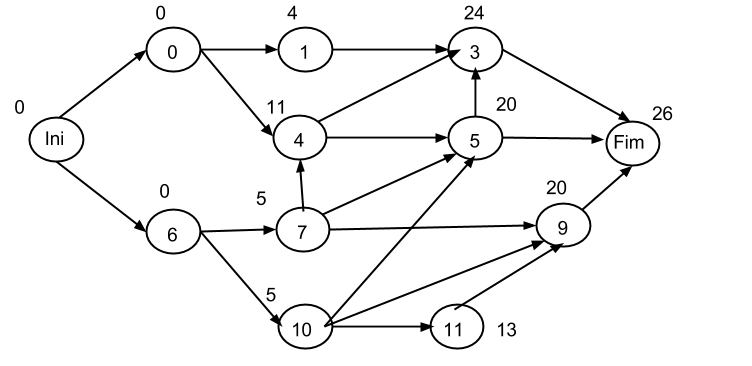
\includegraphics[scale=0.5]{./img/p2_tempos_inicio} \caption{Grafo com
	tempo de início de cada atividade (em unidades de tempo arbitrárias)}
\label{p2:fig:tempos_inicio}
 \end{figure}


\section{Validação do modelo}

Para validar os resultados, tanto na função objetivo como nas restrições,
substituímos os valores das variáveis de decisão pelo valor que estas tomam na
solução que o \texttt{lp\_solve} indica como ótima. A ideia é verificar que os valores das
variáveis de decisão obtidos confirmam o valor da função objetivo obedecendo
a todas as restrições.

Para evitar ao máximo o erro humano, a substituição de variáveis foi feita
recorrendo a ferramentas que auxiliaram a substituição automática das variáveis
pelo seu valor.

\subsection{Variáveis de decisão}

No resultado obtido, todas as variáveis tomam um valor maior ou igual a 0, tal
como seria de esperar.

\subsection{Função objetivo}

Neste modelo a função objetivo consiste apenas no valor de uma variável,
$T_{fim}$, que vale 26 unidades de tempo na solução ótima. Por motivos que não fazem parte do
âmbito deste trabalho, o valor esperado para a duração mínima
do projeto deverá ser o mesmo valor de duração encontrado no caminho crítico da
Parte I. O valor obtido corresponde de facto ao esperado, uma vez que a duração do
caminho crítico obtido na Parte I foi também igual a 26 unidades de tempo.


\subsection{Restrições}


\begin{verbatim} 

//Nodo Inicial
Tini >= 0 + 0;
0 >= 0 + 0;

//Nodo 0
T0 >= Tini + 0; 
0 >= 0 + 0;

//Nodo 1
T1 >= T0 + 4; 
4 >= 0 + 4;

//Nodo 3
T3 >= T1 + 6; 
24 >= 4 + 6;

T3 >= T5 + 4; 
24 >= 20 + 4;

T3 >= T4 + 9; 
24 >= 11 + 9;

//Nodo 4
T4 >= T0 + 4; 
11 >= 0 + 4;

T4 >= T7 + 6; 
11 >= 5 + 6;

//Nodo 5
T5 >= T4 + 9; 
20 >= 11 + 9;

T5 >= T7 + 6; 
20 >= 5 + 6;

T5 >= T10 + 8; 
20 >= 5 + 8;

//Nodo 6
T6 >= Tini + 0; 
0 >= 0 + 0;

//Nodo 7
T7 >= T6 + 5; 
5 >= 0 + 5;

//Nodo 9
T9 >= T7 + 6; 
20 >= 5 + 6;

T9 >= T11 + 7; 
20 >= 13 + 7;

T9 >= T10 + 8; 
20 >= 5 + 8;

//Nodo 10
T10 >= T6 + 5; 
5 >= 0 + 5;

//Nodo 11
T11 >= T10 + 8; 
13 >= 5 + 8;

//Nodo final
Tfim >= T3 + 2; 
26 >= 24 + 2;

Tfim >= T5 + 4; 
26 >= 20 + 4;

Tfim >= T9 + 2; 
26 >= 20 + 2;

\end{verbatim}

Assim conclui-se que todas as restrições são respeitadas.

